\documentclass{article}
\usepackage[utf8]{inputenc}
\usepackage{graphicx}
\usepackage{tikz}
\usepackage{listings}
\usepackage{xcolor}

\definecolor{codegreen}{rgb}{0,0.6,0}
\definecolor{codegray}{rgb}{0.5,0.5,0.5}
\definecolor{codepurple}{rgb}{0.58,0,0.82}
\definecolor{backcolour}{rgb}{0.95,0.95,0.92}

\lstdefinestyle{mystyle}{
    backgroundcolor=\color{backcolour},   
    commentstyle=\color{codegreen},
    keywordstyle=\color{magenta},
    numberstyle=\tiny\color{codegray},
    stringstyle=\color{codepurple},
    basicstyle=\ttfamily\footnotesize,
    breakatwhitespace=false,         
    breaklines=true,                 
    captionpos=b,                    
    keepspaces=true,                 
    numbers=left,                    
    numbersep=5pt,                  
    showspaces=false,                
    showstringspaces=false,
    showtabs=false,                  
    tabsize=2
}

\lstset{style=mystyle}
\renewcommand{\lstlistingname}{Algoritmo}

\title{Programa 1: Universo}
\author{Dueñas Jiménez Cristian Alexis}

\begin{document}
\maketitle

\section{Introducción}
Como bien hemos visto en clase, un autómata es un modelo computacional que consiste en un conjunto de estados bien definidos, un estado inicial, un alfabeto de entrada y una función de transición. El problema consta de encontrar el Universo(cantidad de combinaciones posibles de cadenas dado un alfabeto) dada una $N$. Como se nos plantea, el alfabeto es binario, con el uno y el cero como únicos caracteres. La $N$ representa la longitud en bits máxima que se pueden encontrar en el Universo. Para encontrar esto, se hace uso de la suma binaria. Se suma de uno en uno, para encontrar todas las combinaciones posibles. Sin embargo, hay algunas combinaciones que no se reflejan únicamente sumando de uno en uno. 
\section{Marco Teórico}
Un autómata es un modelo matemático para una máquina de estado finito, en el que dada una entrada de símbolos, «salta» mediante una serie de estados de acuerdo a una función de transición (que puede ser expresada como una tabla). Esta función de transición indica a qué estado cambiar dados el estado actual y el símbolo leído. Su universo está dado por todas las posibilidades que puede encontrar un autómata dado un lenguaje.
\section{Desarrollo}
Para encontrara todas las combinaciones posibles, implementamos una función llamada $sigma$ que tiene como parámetro la $N$ que ingresa el usuario. 

Primero, se hace uso de listas para guardar datos que nos serán de utilidad para posteriormente graficar nuestros datos.

\begin{lstlisting}[language=Python, caption=Implementación del Universo]
import matplotlib.pyplot as plt
import numpy as np
import os
import sys

def graficar(largo, unos, ejeX, ejeY):
    
    plt.plot(largo, unos, marker="")
    plt.xlabel(ejeX)
    plt.ylabel(ejeY)
    plt.title("GRAFICA")
    plt.show()

def sigma(n):

    unos = [] #Arreglo para almacenar la cantidad de unos en cada cadena binaria.
    largo =[] #Arreglo para determinar cuantas cadenas se generan
    cont = -1 #Contador el cual incrementa con cada iteración de los fors.
    concat = ""
    countElements = 0
    newString = ""
    unos64 = []
    cadenas64 = 0
    largo64 = []
    f1 = open("../PARCIAL 1/PROGRAMAS/Programa1/outputs/universo.txt", "w", encoding="utf-8") 
    f2 = open("../PARCIAL 1/PROGRAMAS/Programa1/outputs/Concatenadas.txt", "w", encoding="utf-8")
    f3 = open("../PARCIAL 1/PROGRAMAS/Programa1/outputs/Segmentadas.txt", "w", encoding="utf-8")
    f1.write("{") 

    for a in range(n+1): ##Generamos nuestro bucle, este sólo es para imprimir la cantidad de iteraciones que se llevan a cabo. Ponemos n+1, ya que 
        print("n = ",a) #Imprimimos las iteraciones realizadas, conforme se va realizando cada una de ellas.
        for x in range(2 ** a): #En este segundo for, determinamos la cantidad de cadenas que habrá según el valor de a, es decir, según el número de iteración. Esto se determina con 2^a.
            
            cont += 1 #Incrementamos el contador que inicializamos anteriormente, esto para llevar el conteo de cadenas.
            binario = bin(x)[2:] 
            
            if len(binario) < a: #Condición para agregar ceros.
                binario = ('0' * (a-len(binario))) + binario 
            
            if a == 0: 
                binario = 'ε' #Cuando nuestro valor ingresado es "0", el universo se determina con su respectivo símbolo.

            if a > 0:
                concat = concat+binario

            f1.write(binario + ',') #Mandamos a escribir en nuestro archivo cada una de las cadenas generadas.
            unos.append(binario.count('1')) #Realizamos el conteo de 1's en cada cadena y lo guardamos en el arreglo de unos.
            largo.append(cont) #Almacenamos la cantidad de cadenas que van en cada iteración

    f2.write(concat)
    f2.close()
    f1.write("}") #Una vez finalizados los ciclos, cerramos nuestro conjunto con una llave.
    f1.close() #Cerramos el archivo
    f3.write("Segmnentadas" + os.linesep)

    for char in concat:
        countElements+=1
        newString = newString+char
        
        if countElements == 64:
            cadenas64 += 1
            unos64.append(newString.count('1'))
            largo64.append(cadenas64)
            countElements = 0
            f3.write(newString + os.linesep)
            newString = ""

    graficar(largo,unos, "Cantidad de Cadenas", "Cantidad de 1's") #Mandamos llamar la función graficar, la cual nos muestra la cantidad de 1's en cada cadena, por lo cual le mandamos la variable largo y unos.
    graficar(largo,np.log10(unos), "Cantidad de Cadenas", "Cantidad de 1's (Log10)")
    graficar(largo64,unos64, "Cantidad de Cadenas", "Cantidad de 1's")
    graficar(largo64,np.log10(unos64), "Cantidad de Cadenas", "Cantidad de 1's (Log10)")

#Generamos nuestro menú de opciones
opc = "1"
print("MENU DE OPCIONES")
while opc == "1":
    
    opc = input("Seleccione una opción: \n1.- Ingresar n \n2.- Finalizar\n")
    
    if opc == "1":
        n = int(input("Ingrese el valor de n: "))
        sigma(n)
    else:
        if opc == "2":
            print(f"FIN DE LA EJECUCION")
            sys.exit(0)
        else:
            if opc != "1":
                print("Seleccione una opcion valida")


\end{lstlisting}
El primer ciclo, nos ayuda a saber en que $n$ nos encontramos. En otras palabras, nos dice la cantidad de bits que vamos a tener en la cadena generada. El segundo for hace uso de la suma binaria. Aumenta de uno en uno los elementos.
\newline\newline
La sentencia $if len(binario) < a:$ nos permite agregar ceros a la izquierda para tener una cadena que sea existente dentro de la cantidad de bits. Para entenderlo mejor, supongamos que el usuario ingresa $n = 3$. El primer ciclo for irá de 0 a 3. En la primera iteración, la longitud en bits máxima que puede tener la cadena es 0. En la segunda iteración, la longitud ahora es de uno. Entra en el segundo for, donde despliega todos las combinaciones posibles cuando $n=1$. Al terminar el ciclo, $n=2$. Entra de nuevo en el segundo for donde mostrará de nuevo las combinaciones posibles. Sin embargo, al convertir los decimales en binario, no toma en cuenta la condición de la longitud. Para que esto se cumpla, resta la cantidad esperada de bits, menos la longitud de la cadena la arrojada al convertir de decimal a binario. El resultado de eso es la cantidad de ceros a la izquierda que se la agrega a la cadena. De esta forma, se garantiza que el programa no tendrá cadenas repetidas. Una vez obtenida la cadena, la escribe en el archivo. Del mismo modo, guarda en arreglos la cantidad de unos en la cadena, el total de caracteres en la cadena, y la cantidad de cadenas encontradas al momento. 
Además, cada que se genera una cadena, se va concatenando para que al final forme una sola, establecemos una condición para que no se agregue el símbolo de Epsilon en la cadena. Una vez que tenemos la cadena unida, la recorremos para formar cadenas de 64 bits.
\newline\newline
Para graficar, hacemos uso de la librería matplotlib. El programa tiene una función la cual se reciben los arreglos llenados en la función sigma, que usa para representarlos en la gráfica. 
Dado que el archivo generado para n=27 es muy grande y ocupa mucho espacio, se tomó una prueba con n=20, donde el archivo sí es manejable.

\subsection{Implementación}
\begin{center}
    \includegraphics[scale = 0.7]{universoFile1.PNG}
    \caption{Archivo Generado}
\end{center}

\begin{center}
    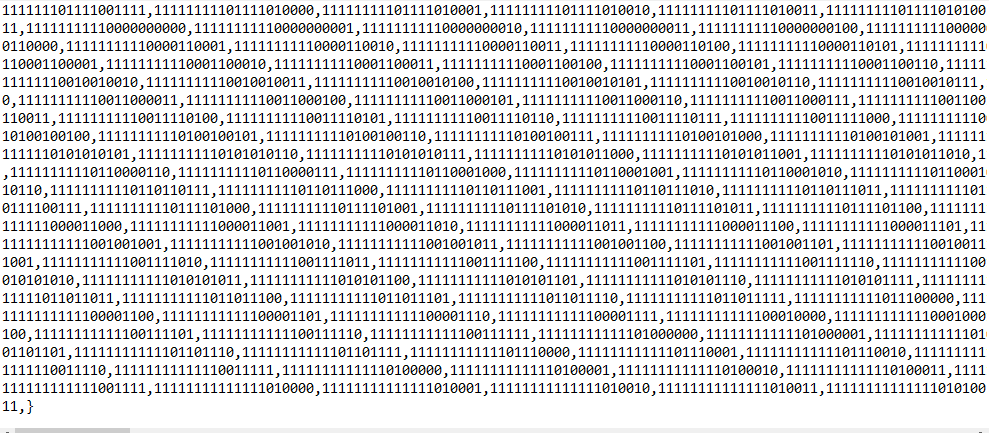
\includegraphics[scale = 0.7]{UniversoFile2.png}
    \caption{}
\end{center}

\begin{center}
    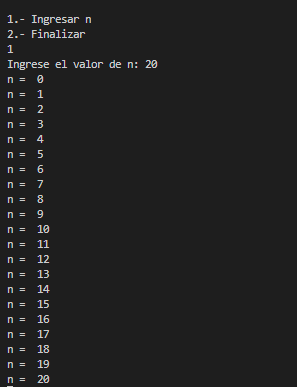
\includegraphics[scale = 0.7]{console.png}
    \caption{Consola}
\end{center}

\begin{center}
    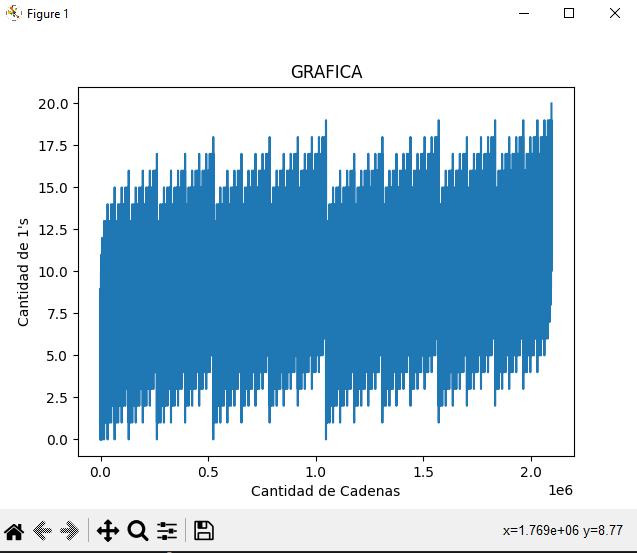
\includegraphics[scale = 0.7]{graphic1.png}
    \caption{Grafica 1)}
\end{center}

\begin{center}
    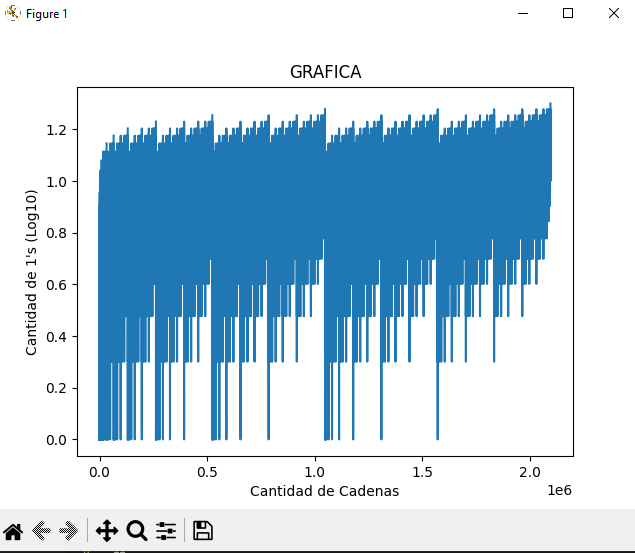
\includegraphics[scale = 0.7]{graphic2.png}
    \caption{Grafica 2}
\end{center}

\begin{center}
    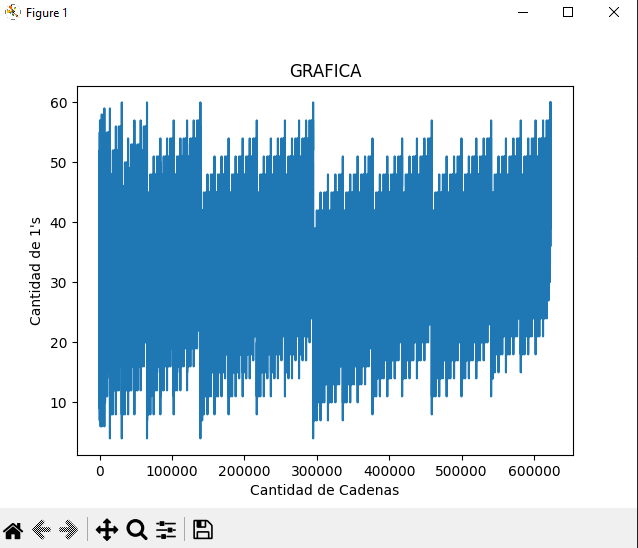
\includegraphics[scale = 0.7]{graphic3.png}
    \caption{Grafica 3 (Cadenas de 64 bits)}
\end{center}

\begin{center}
    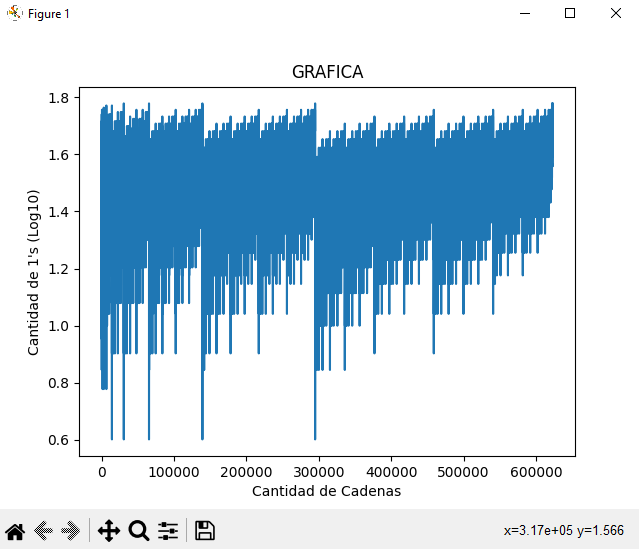
\includegraphics[scale = 0.7]{graphic4.png}
    \caption{Grafica 4 (Cadenas de 64 bits)}
\end{center}

\begin{center}
    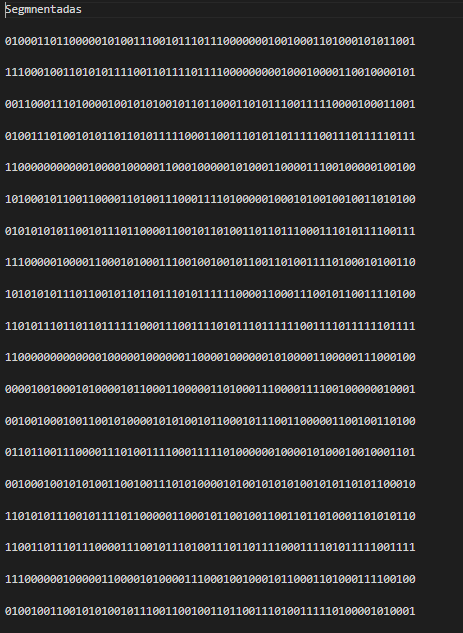
\includegraphics[scale = 1]{segments.png}
    \caption{Cadenas de 64 bits}
\end{center}

\begin{thebibliography}{}
    \bibitem{automata}
    Sánchez, E. H. (2019). Lic. en Informática. Unidad de Apoyo para el Aprendizaje. https://programas.cuaed.unam.mx/repositorio/moodle/pluginfile.php/1163/modresource/content
    /1/contenido/index.html#
    \bibitem{nreinas2}
    GeeksforGeeks. (2019, 16 octubre). N Queen Problem | Backtracking-3. https://www.geeksforgeeks.org/n-queen-problem-backtracking-3/?ref=rp
    \bibitem{reina_movi}
    Ocho reinas reina atacarr.JPG. (2006, 20 mayo). [Imagen]. Wikipedia. https://upload.wikimedia.org/wikipedia/commons/d/d6/Ocho\_reinas\_reina\_atacarr.JPG
    \bibitem{reina_ata}
    Ocho reinas reina atacar fila. (2006, 10 mayo). [Imagen]. Wikipedia. https://upload.wikimedia.org/wikipedia/commons/a/ad/Ocho\_reinas\_reina\_atacar\_fila.JPG
    \bibitem{backtracking}
    GeeksforGeeks. (2021, 9 febrero). Backtracking | Introduction. https://www.geeksforgeeks.org/backtracking-introduction/
    \bibitem{arbol_back}
    Backtracking. (s. f.). [Imagen]. InterviewBit. https://ibpublicimages.s3-us-west-2.amazonaws.com/tutorial/backtracking1.pngFigura 2
    \bibitem{arbol_reina}
    [Árbol de búsqueda del problema de las 4 reinas]. (2015, 5 febrero). Ivan Voroshilin’s Blog. https://ivoroshilin.files.wordpress.com/2015/02/backtrack.png
\end{thebibliography}

\end{document}